\normaltrue \difficilefalse \tdifficilefalse
\correctiontrue

%\UPSTIidClasse{11} % 11 sup, 12 spé
%\newcommand{\UPSTIidClasse}{11}

\exer{Identification temporelle $\star$ \label{B2:06:502}}
\setcounter{numques}{0}
\UPSTIcompetence[2]{B2-06}
\index{Compétence B2-06}
\index{Identification}
\index{Identification temporelle}
\index{Ordre 1}
\index{Ordre 2}
\ifcorrection
\else
\textbf{Pas de corrigé pour cet exercice.}
\fi


\ifprof 
\else
Soit la réponse à un échelon.
\begin{center}
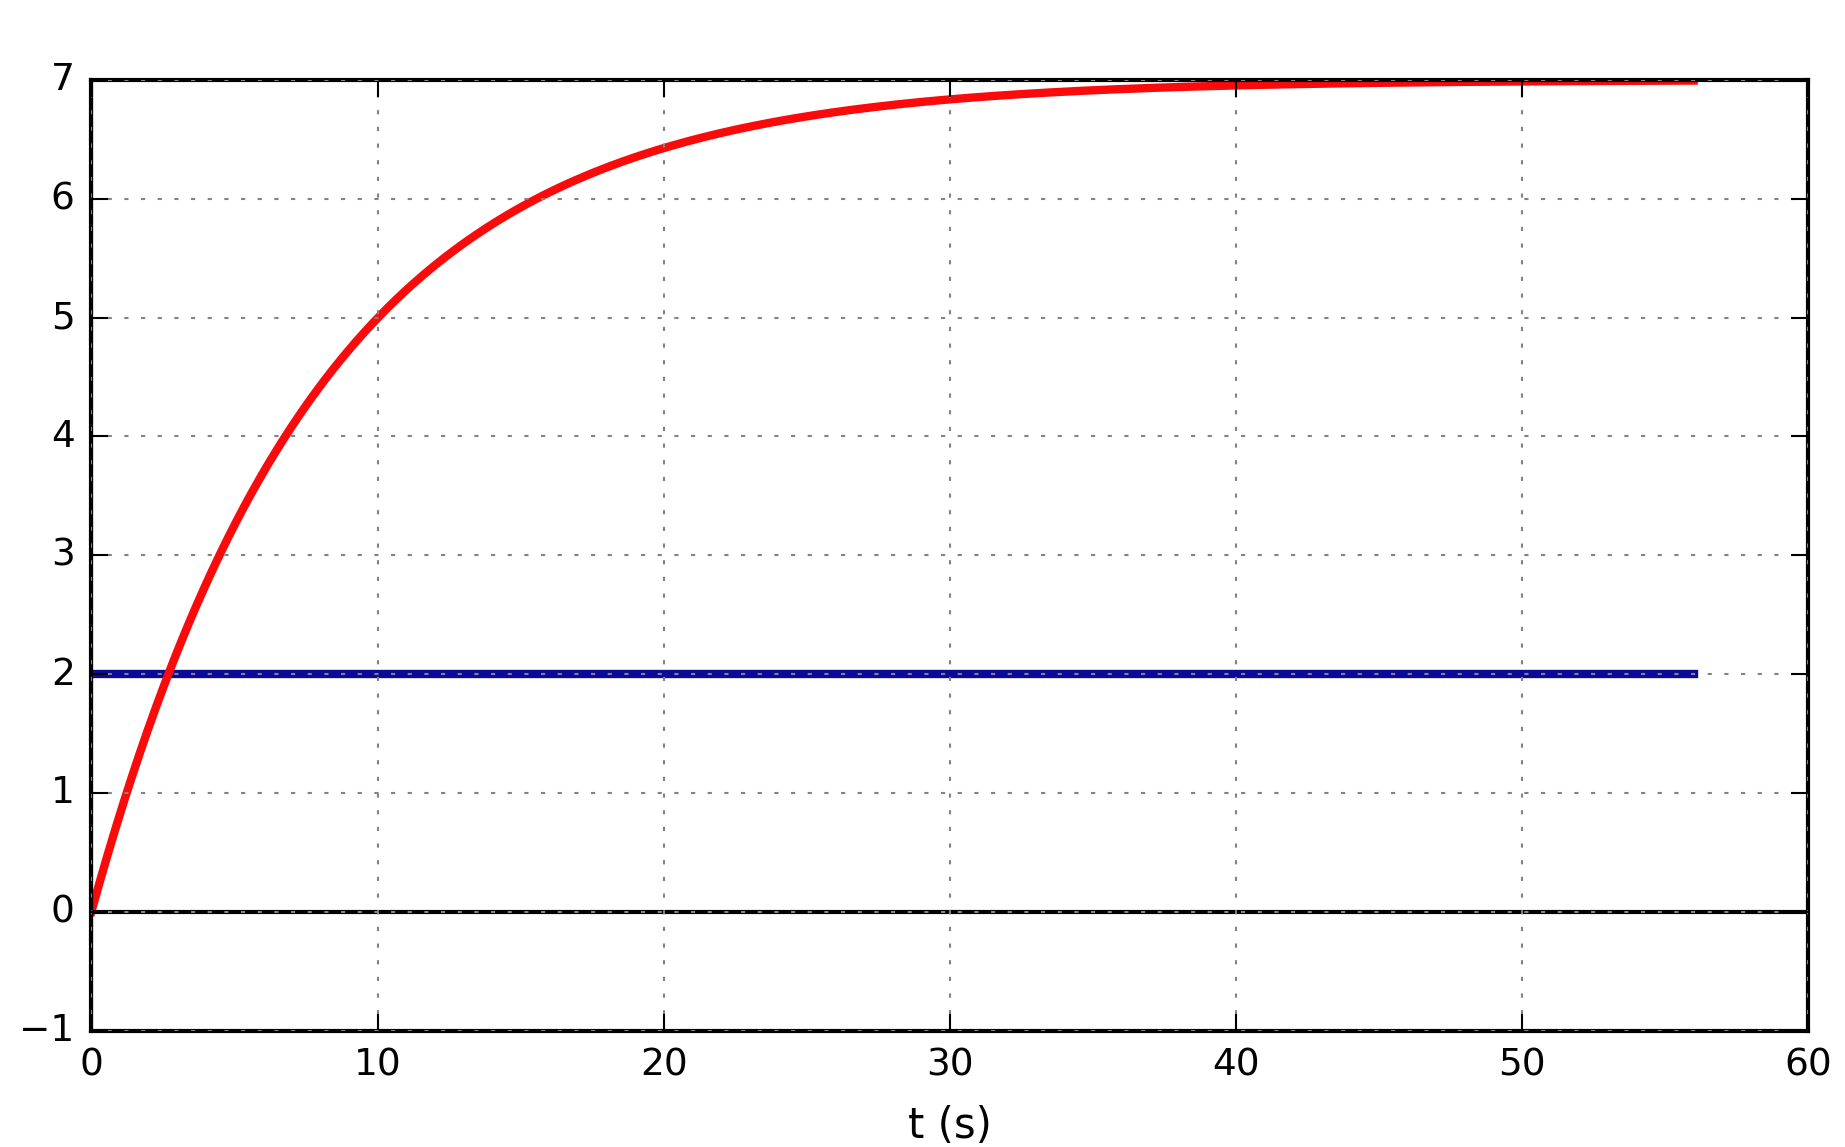
\includegraphics[width=.9\linewidth]{502_01}
\end{center}
\fi

\question{Déterminer la fonction de transfert du système.}
\ifprof
\begin{center}
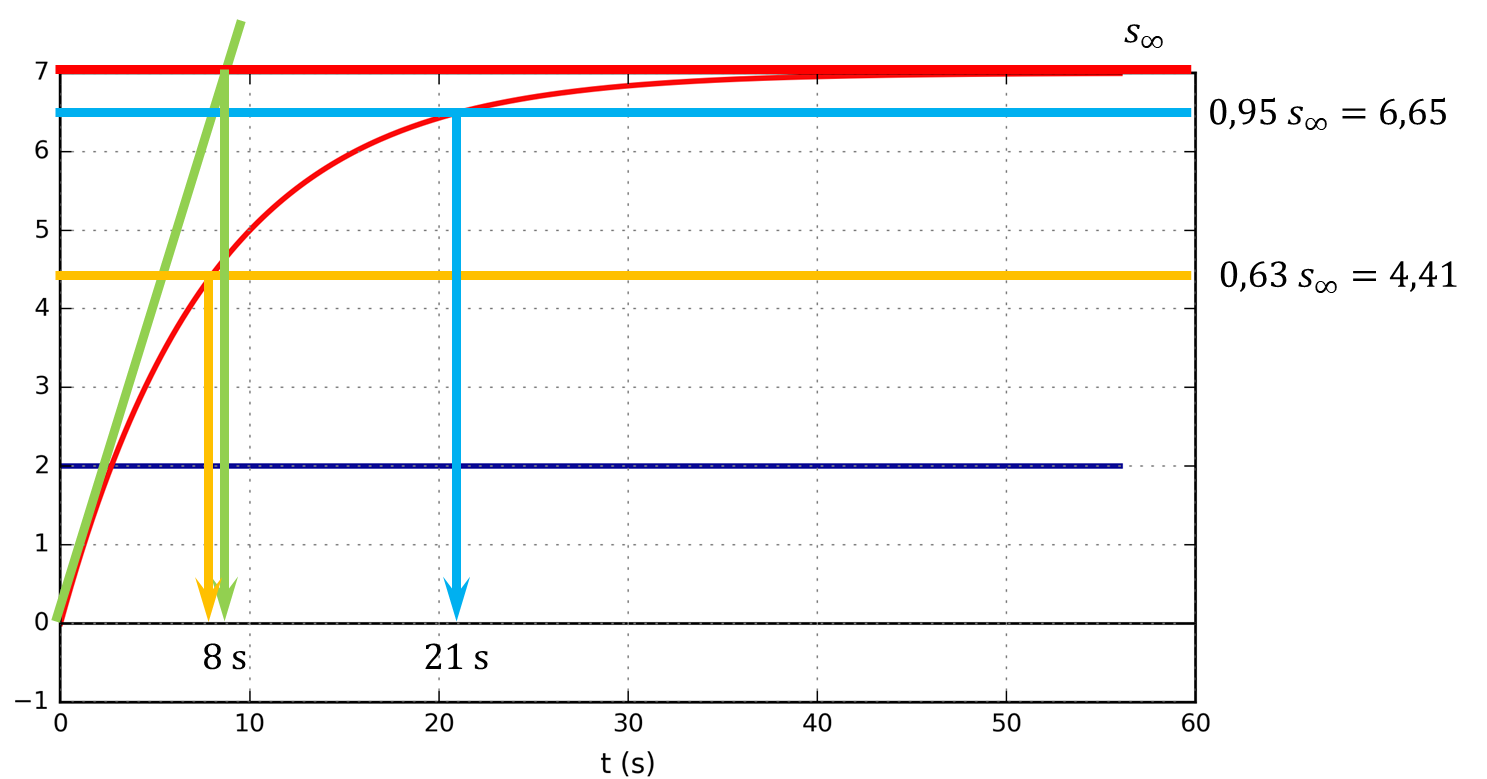
\includegraphics[width=8cm]{502_01_cor}
\end{center}

La tangente à l'origine est non nulle. Il n'y a pas de dépassement. On va donc identifier un système d'ordre 1 de la forme $H(p)=\dfrac{K}{1+\tau p}$.

L'échelon d'entrée a une amplitude de 2. En régime permanent la valeur atteinte est de 7. On a donc $K = \dfrac{7}{2}=3,5$.

Pour identifier la constante de temps, on peut : 
\begin{itemize}
\item regarder à quel temps a lieu l'intersection entre l'asympote en régime permanent et la tangente à l'origine;

\item mesurer le temps de temps réponse à 63\,\%;

\item mesurer le temps de temps réponse à 95\,\% et diviser cette valeur par 3.
\end{itemize}

On a donc $H(p)=\dfrac{3,5}{1+8p}$.
\else
\fi



\ifprof 
\else
Soit la réponse à un échelon d'amplitude 2,5.

\begin{center}
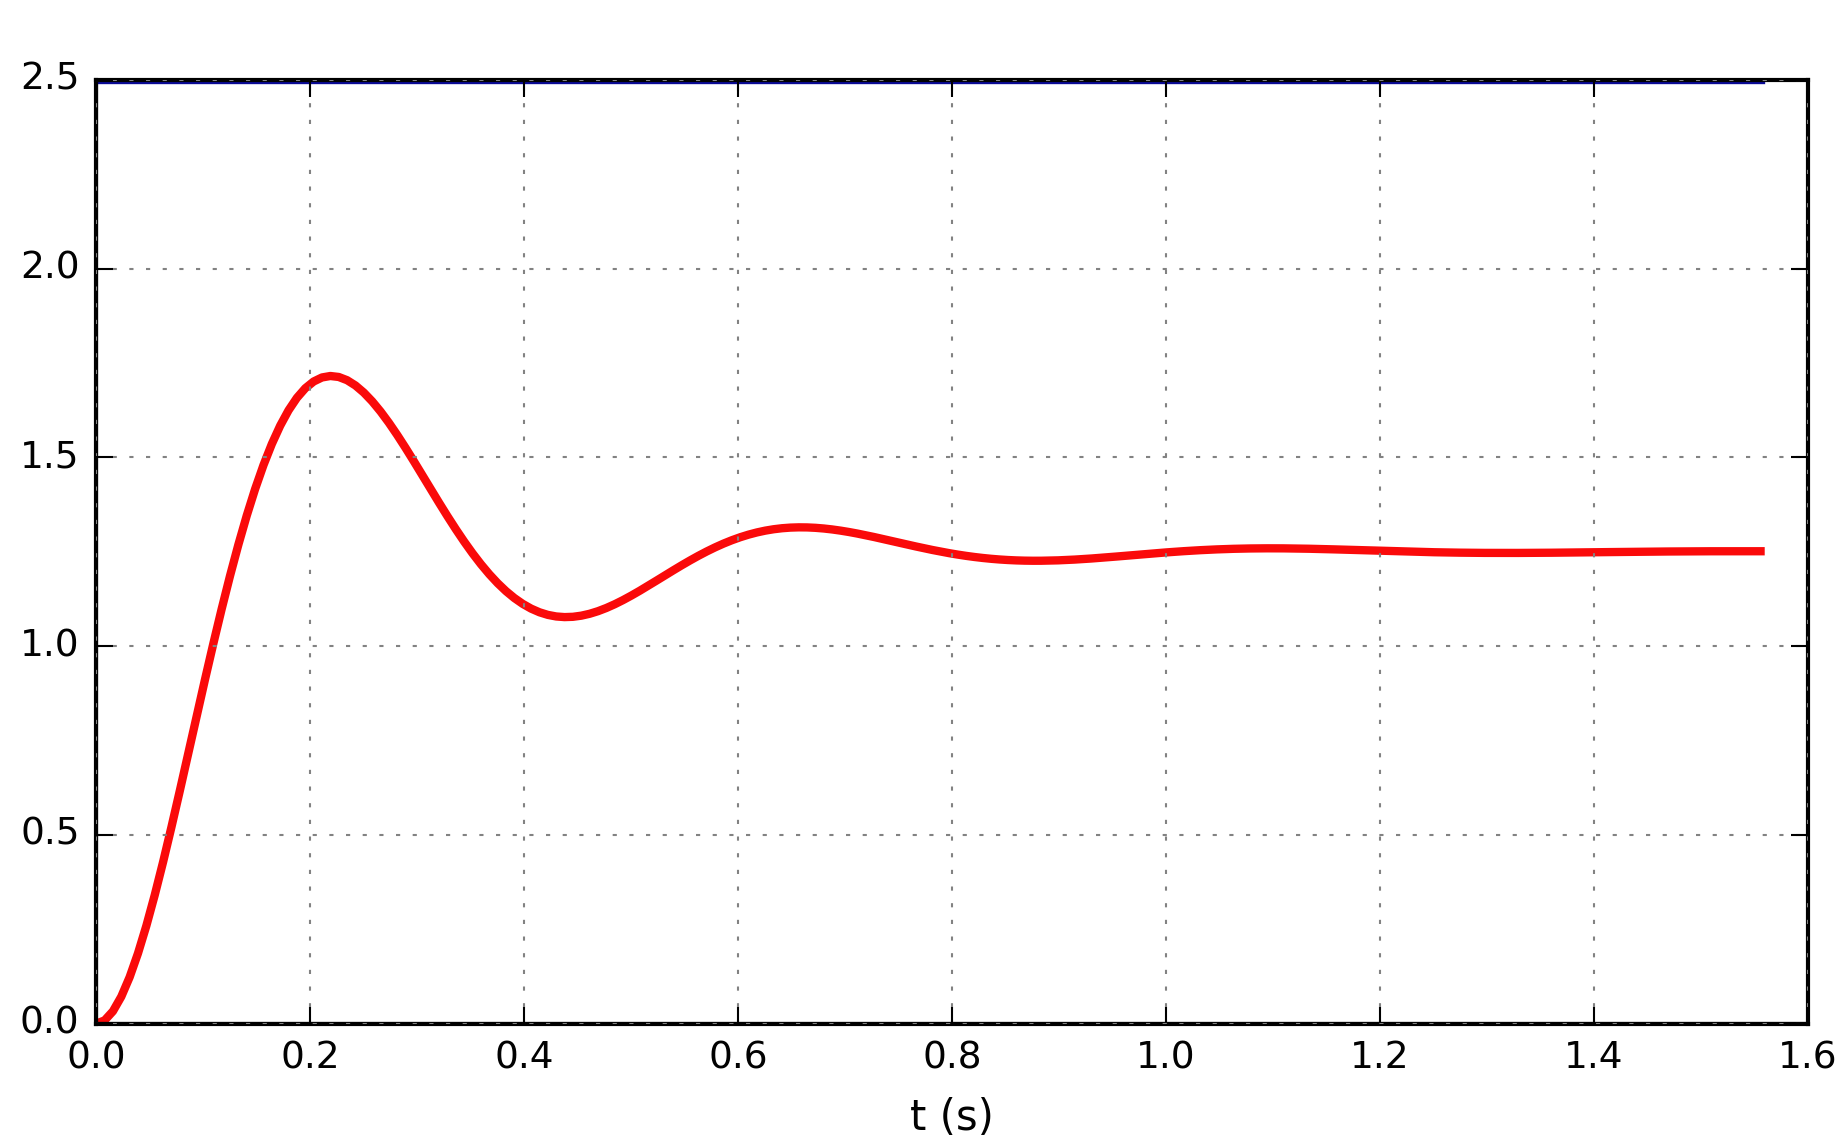
\includegraphics[width=.9\linewidth]{502_02}
\end{center}
\fi

\question{Déterminer la fonction de transfert du système en réalisant les mesures nécessaires et en utilisant les formules appropriées.}
\ifprof
\begin{center}
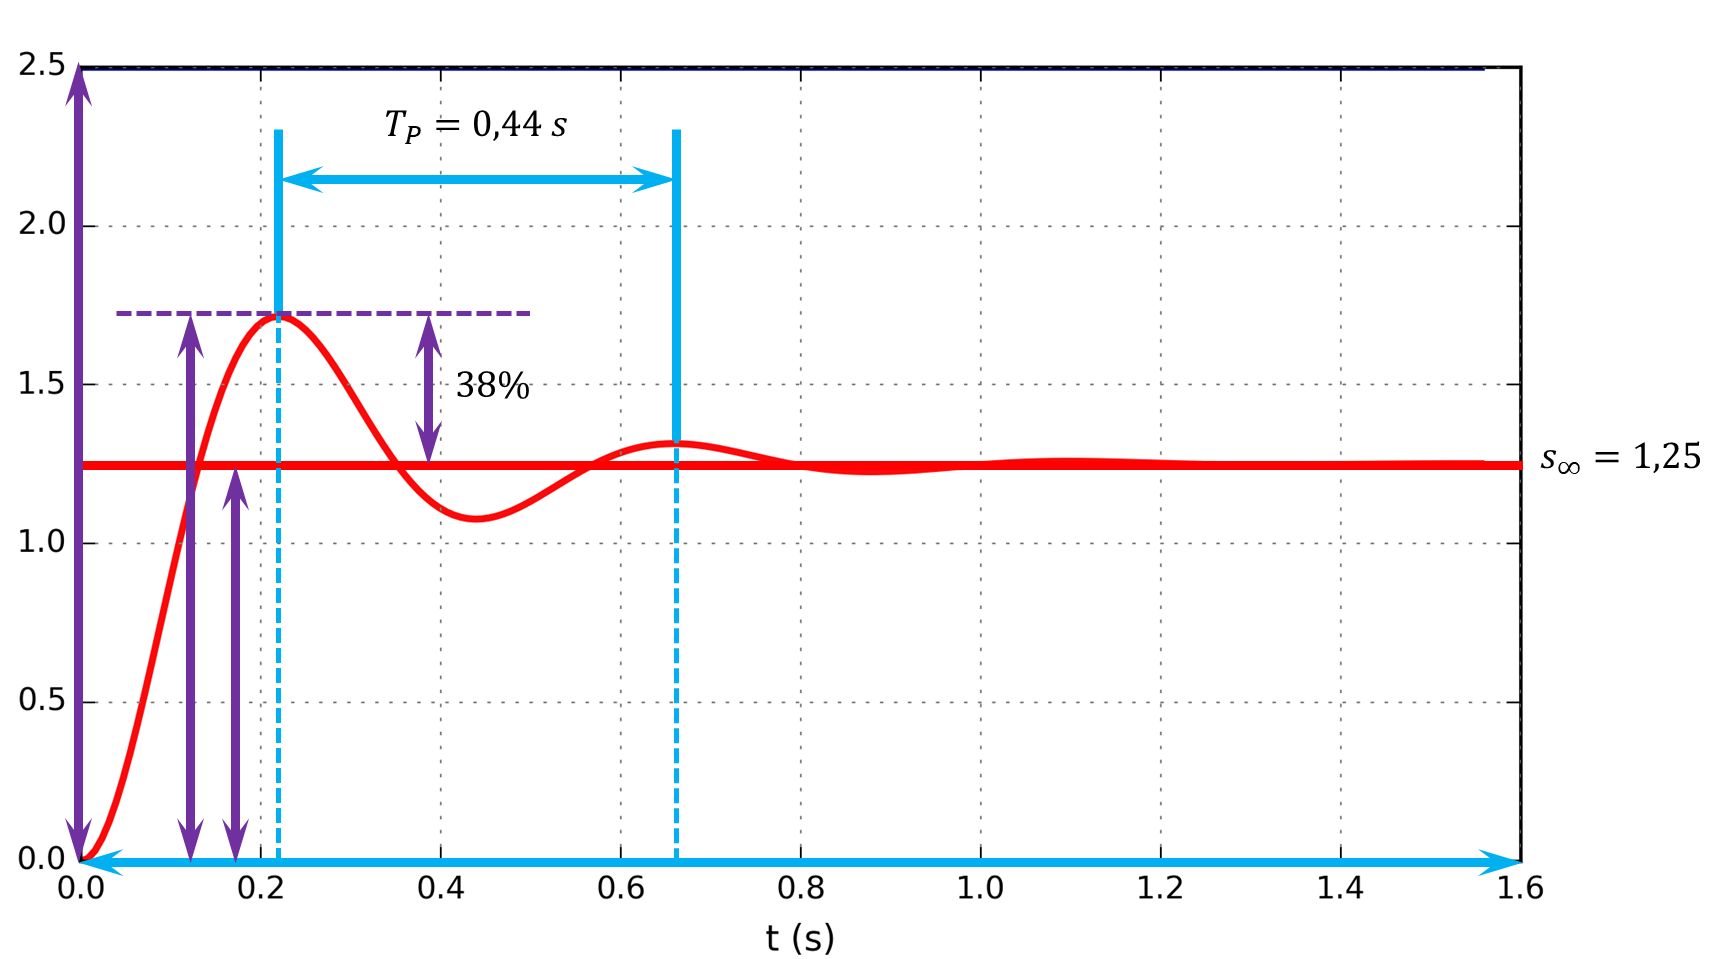
\includegraphics[width=8cm]{502_02_cor}
\end{center}

La tangente à l'origine est nulle et il y a des dépassements. On modélise le système par un système d'ordre 2. 
$H(p)=\dfrac{K}{1+\dfrac{2\xi}{\omega_0}p+\dfrac{p^2}{\omega_0^2}}$.

On a $K= \dfrac{1,25}{2,5}=0,5$.


On mesure un dépassement de 
$1,38 = e^{\dfrac{-\pi \xi}{\sqrt{1-\xi^2}}}$
$\Leftrightarrow \ln 0,38 = \dfrac{-\pi \xi}{\sqrt{1-\xi^2}}$
$\Leftrightarrow \sqrt{1-\xi^2} \ln 1,38 = -\pi \xi$
$\Leftrightarrow (1-\xi^2) (\ln 1,38)^2= \pi^2 \xi^2$
$\Leftrightarrow (\ln 1,38)^2-\xi^2(\ln 1,38)^2 = \pi^2 \xi^2$
$\Leftrightarrow (\ln 1,38)^2 = \pi^2 \xi^2 + \xi^2(\ln 1,38)^2$
$\Leftrightarrow (\ln 1,38)^2 =\xi^2 \left(\pi^2  + (\ln 1,38)^2\right)$
$\Leftrightarrow \dfrac{(\ln 1,38)^2}{\pi^2  + (\ln 1,38)^2} =\xi^2 $
$\Leftrightarrow \xi = \sqrt{\dfrac{(\ln 1,38)^2}{\pi^2  +(\ln 1,38)^2}} =0,3 $.


Par ailleurs, $\omega_0 = \dfrac{2\pi }{T_p \sqrt{1-\xi^2}} =\dfrac{2\pi }{0,44 \sqrt{1-0,3^2}} = \SI{14,9}{rad.s^{-1}}$.

Au final, $H(p)=\dfrac{0,5}{1+\dfrac{2\times 0,3}{14,9}p+\dfrac{p^2}{14,9^2}}$.


\else
\fi



\question{Déterminer la fonction de transfert du système en utilisant les abaques.}
\ifprof
Le dépassement est de 38 \%. On a donc $\xi = 0,3$.

De plus, on mesure $T_{5\%}\times \omega_0 =8$ avec $T_{5\%}=\SI{0,51}{s}$ on a $\omega_0 = 8/0,5 \simeq \SI{16}{rad.s^{-1}}$.

Au final, $H(p)=\dfrac{0,5}{1+\dfrac{2\times 0,3}{16}p+\dfrac{p^2}{16^2}}$.
\begin{center}
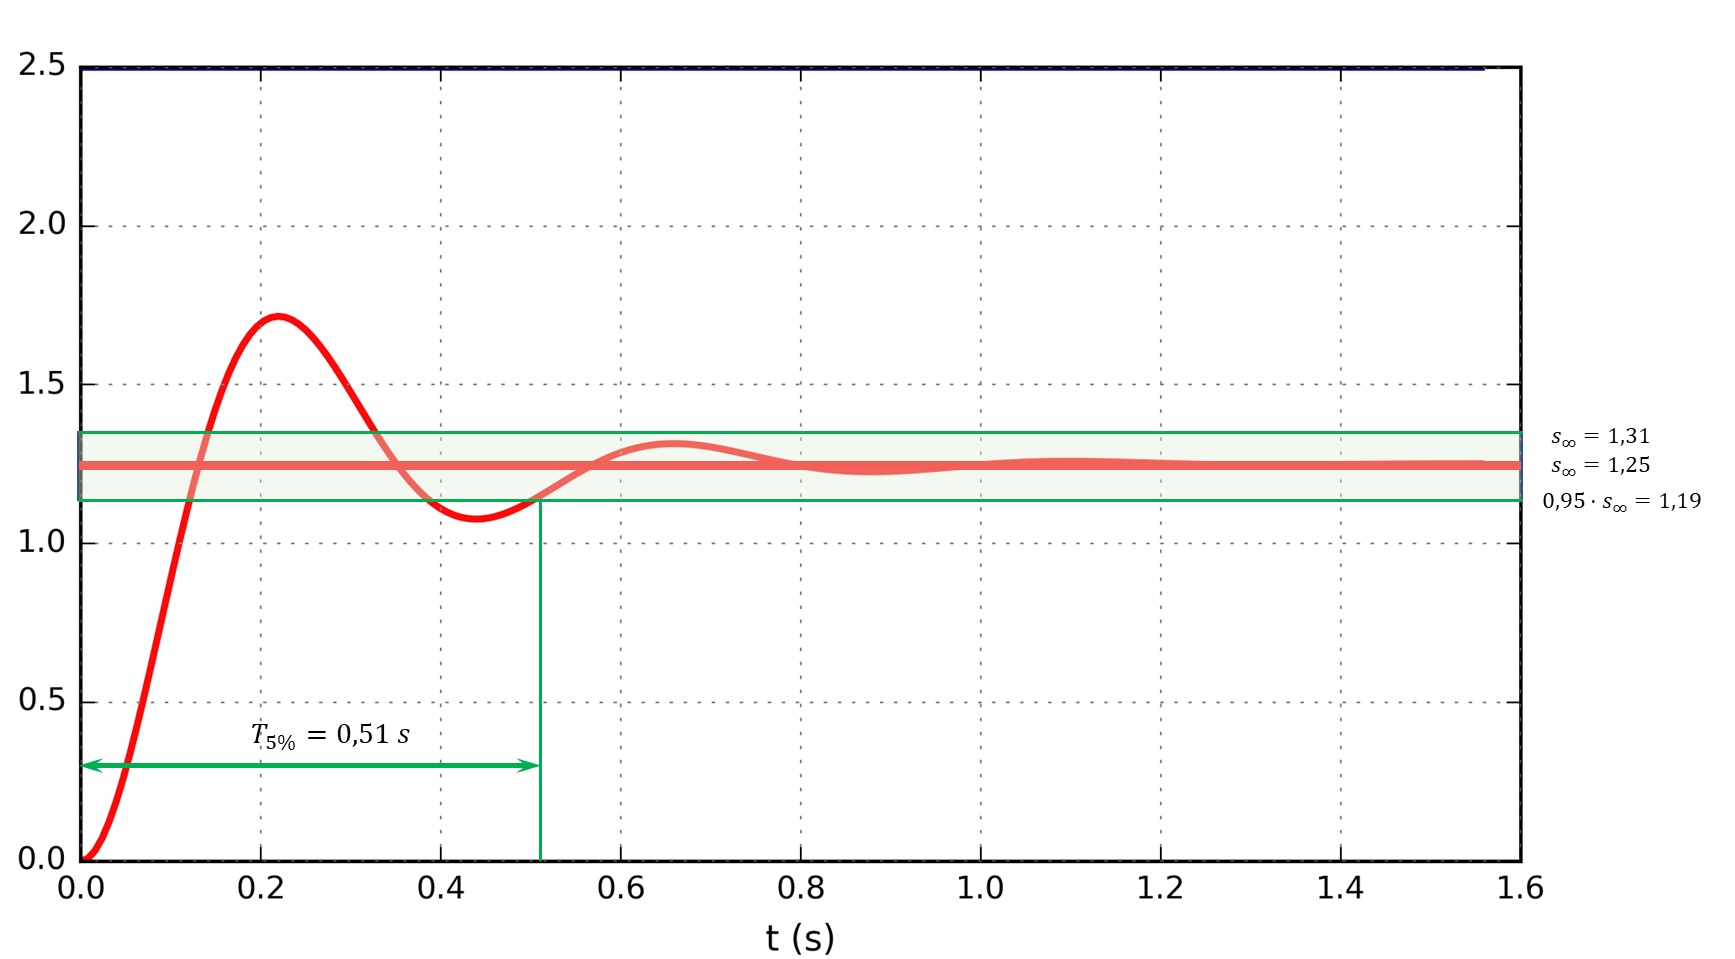
\includegraphics[width=8cm]{502_03_cor}
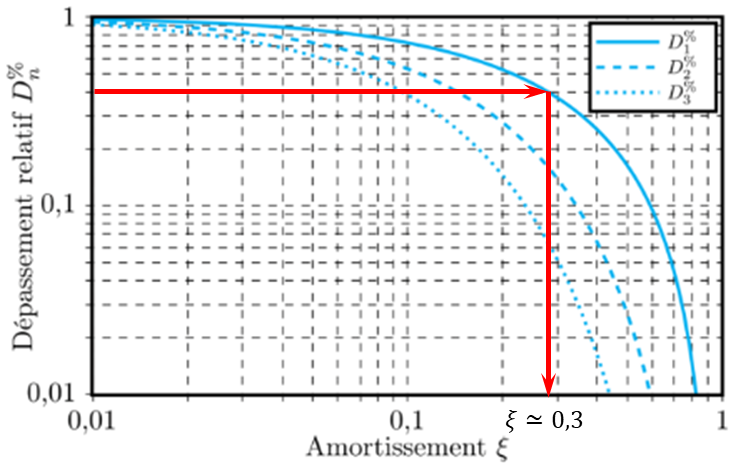
\includegraphics[width=8cm]{502_04_cor}
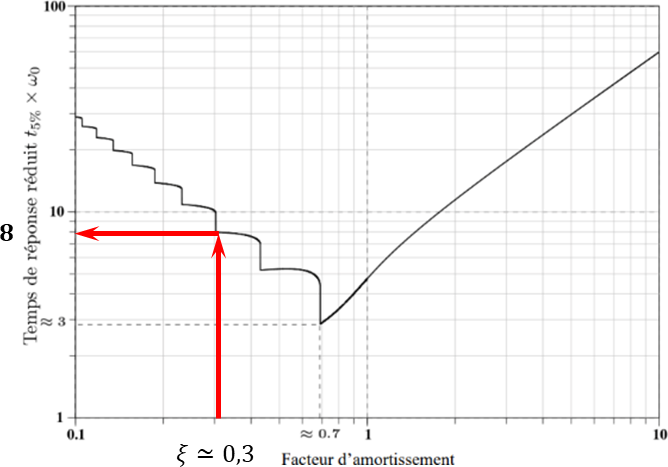
\includegraphics[width=8cm]{502_05_cor}
\end{center}
\else
\begin{center}
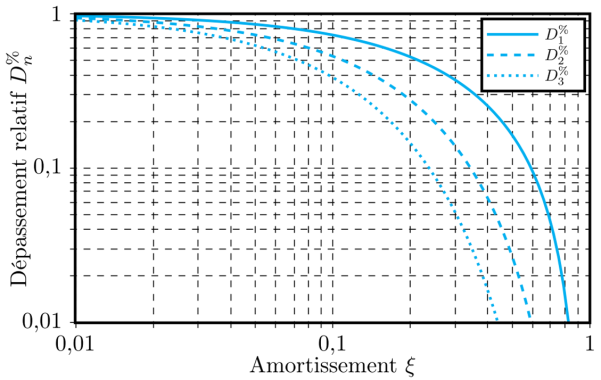
\includegraphics[width=8cm]{502_03}
\end{center}
\begin{center}
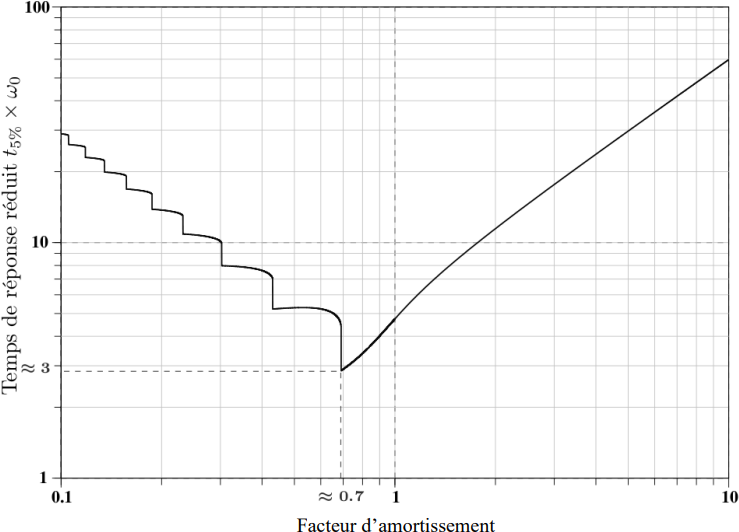
\includegraphics[width=8cm]{502_04}
\end{center}
\fi


\ifprof
\else
\footnotesize
\begin{tabular}{|p{.9\linewidth}|}
\hline
Indications :
\begin{enumerate}
\item  $H(p)=\dfrac{3,5}{1+8p}$.
\item $H(p)=\dfrac{0,5}{1+\dfrac{2\times 0,1}{14,25}p+\dfrac{p^2}{14,25^2}}$.
\item $H(p)=\dfrac{0,5}{1+\dfrac{2\times 0,3}{16}p+\dfrac{p^2}{16^2}}$.
\end{enumerate} \\ \hline
\end{tabular}
\normalsize

\begin{flushright}
\footnotesize{Corrigé  voir \ref{B2:06:502}.}
\end{flushright}%
\fi